% !Mode:: "TeX:UTF-8"
\def\usewhat{dvipdfmx}                              % 定义编译方式 dvipdfmx 或者 pdflatex ,默认为 dvipdfmx
                                                    % 方式编译,如果需要修改,只需改变花括号中的内容即可。
\documentclass[12pt,openright,twoside]{book}
                                                    % 博士论文通常采用双页排版
% !Mode:: "TeX:UTF-8"
%  Authors: 张井   Jing Zhang: prayever@gmail.com     天津大学2010级管理与经济学部信息管理与信息系统专业硕士生
%           余蓝涛 Lantao Yu: lantaoyu1991@gmail.com  天津大学2008级精密仪器与光电子工程学院测控技术与仪器专业本科生
%  Supplementer:Jack Shen: congshen@tju.edu.cn        天津大学2015级计算机科学与技术学院计算机应用技术专业博士生
%%%%%%%%%% Package %%%%%%%%%%%%
\usepackage{graphicx}                       % 支持插图处理
%\usepackage[a4paper,text={150true mm,224true mm},top=35.5true mm,left=30true mm,head=5true mm,headsep=2.5true mm,foot=8.5true mm]{geometry}
\usepackage[a4paper,text={146.6true mm,244.1true mm},top=27.5true mm,left=35.7true mm,head=2.5true mm,headsep=12.5true mm,foot=7.9true mm]{geometry}
                                            % 支持版面尺寸设置
\usepackage{titlesec}                       % 控制标题的宏包
\usepackage{titletoc}                       % 控制目录的宏包
\usepackage{fancyhdr}                       % fancyhdr宏包 支持页眉和页脚的相关定义
\usepackage[UTF8]{ctex}                     % 支持中文显示
\usepackage{color}                          % 支持彩色
\usepackage{amsmath}                        % AMSLaTeX宏包 用来排出更加漂亮的公式
\usepackage{amssymb}                        % 数学符号生成命令
\usepackage[below]{placeins}                %允许上一个section的浮动图形出现在下一个section的开始部分,还提供\FloatBarrier命令,使所有未处理的浮动图形立即被处理
\usepackage{flafter}                        % 使得所有浮动体不能被放置在其浮动环境之前,以免浮动体在引述它的文本之前出现.
\usepackage{multirow}                       % 使用Multirow宏包,使得表格可以合并多个row格
\usepackage{booktabs}                       % 表格,横的粗线;\specialrule{1pt}{0pt}{0pt}
\usepackage{longtable}                      % 支持跨页的表格。
\usepackage{tabularx}                       % 自动设置表格的列宽
\usepackage{subfigure}                      % 支持子图 %centerlast 设置最后一行是否居中
\usepackage[subfigure]{ccaption}            % 支持子图的中文标题
\usepackage[sort&compress,numbers]{natbib}  % 支持引用缩写的宏包
\usepackage{enumitem}                       % 使用enumitem宏包,改变列表项的格式
\usepackage{calc}                           % 长度可以用+ - * / 进行计算
\usepackage{txfonts}                        % 字体宏包
\usepackage{bm}                             % 处理数学公式中的黑斜体的宏包
\usepackage[amsmath,thmmarks,hyperref]{ntheorem}  % 定理类环境宏包,其中 amsmath 选项用来兼容 AMS LaTeX 的宏包
\usepackage{CJKnumb}                        % 提供将阿拉伯数字转换成中文数字的命令
\usepackage{indentfirst}                    % 首行缩进宏包
\usepackage{CJKutf8}                        % 用在UTF8编码环境下,它可以自动调用CJK,同时针对UTF8编码作了设置。
%\usepackage{hypbmsec}                      % 用来控制书签中标题显示内容
\usepackage{algorithm}
\usepackage{listings}%added by cc,  for coding20180316
\usepackage{setspace}%added by cc,  for tablecontents
%\usepackage{algorithmic}
\usepackage{algpseudocode}
\usepackage[all]{xy}
\usepackage{times}%英文使用times new man
\usepackage{mathptmx}%公式中英文使用times new man

% 生成有书签的 pdf 及其生成方式。通常可以在 tjumain.tex 文件的第一行选择 pdflatex 或者是 dvipdfmx 编译手段。如果选择前者,则使用 pdflatex + pdflatex 编译; 如果选择后者,在编译的时候选择 latex + bibtex + latex + latex 编译。出现混淆的时候,系统会报错。

% 如果您的pdf制作中文书签有乱码使用如下命令,就可以解决了
\def\atemp{dvipdfmx}\ifx\atemp\usewhat
\usepackage[dvipdfmx,unicode,               % dvipdfmx 编译, 加入了中文复制,粘贴支持引擎。
            pdfstartview=FitH,
            bookmarksnumbered=true,
            bookmarksopen=true,
            colorlinks=false,
            pdfborder={0 0 1},
            citecolor=blue,
            linkcolor=red,
            anchorcolor=green,
            urlcolor=blue,
            breaklinks=true
            ]{hyperref}
\fi

\def\atemp{pdflatex}\ifx\atemp\usewhat
\usepackage{cmap}                            % pdflatex 编译时,可以生成可复制、粘贴的中文 PDF 文档, 缺点是在Windows上显示时效果不大好,字体发虚
\usepackage[pdftex,unicode,
            %CJKbookmarks=true,
            bookmarksnumbered=true,
            bookmarksopen=true,
            colorlinks=false,
            pdfborder={0 0 1},
            citecolor=blue,
            linkcolor=red,
            anchorcolor=green,
            urlcolor=blue,
            breaklinks=true
            ]{hyperref}
\fi

                               % 定义本文所使用宏包
\graphicspath{{figures/}}                           % 定义所有的 .eps 文件在 figures 子目录下
\begin{document}                                    % 开始全文
\begin{CJK*}{UTF8}{song}                            % 开始中文字体使用
% !Mode:: "TeX:UTF-8"
%  Authors: 张井   Jing Zhang: prayever@gmail.com     天津大学2010级管理与经济学部信息管理与信息系统专业硕士生
%           余蓝涛 Lantao Yu: lantaoyu1991@gmail.com  天津大学2008级精密仪器与光电子工程学院测控技术与仪器专业本科生

%%%%%%%%%% Fonts Definition and Basics %%%%%%%%%%%%%%%%%
\newcommand{\song}{\CJKfamily{song}}    % 宋体
\newcommand{\fs}{\CJKfamily{fs}}        % 仿宋体
\newcommand{\kai}{\CJKfamily{kai}}      % 楷体
\newcommand{\hei}{\CJKfamily{hei}}      % 黑体
\newcommand{\li}{\CJKfamily{li}}        % 隶书
\newcommand{\yihao}{\fontsize{26pt}{26pt}\selectfont}       % 一号, 1.倍行距
\newcommand{\xiaoyi}{\fontsize{24pt}{24pt}\selectfont}      % 小一, 1.倍行距
\newcommand{\erhao}{\fontsize{22pt}{1.25\baselineskip}\selectfont}       % 二号, 1.25倍行距
\newcommand{\xiaoer}{\fontsize{18pt}{18pt}\selectfont}      % 小二, 单倍行距
\newcommand{\sanhao}{\fontsize{16pt}{16pt}\selectfont}      % 三号, 1.倍行距
\newcommand{\xiaosan}{\fontsize{15pt}{15pt}\selectfont}     % 小三, 1.倍行距
\newcommand{\sihao}{\fontsize{14pt}{14pt}\selectfont}       % 四号, 1.0倍行距
\newcommand{\xiaosi}{\fontsize{12pt}{12pt}\selectfont}      % 小四, 1.倍行距
\newcommand{\wuhao}{\fontsize{10.5pt}{10.5pt}\selectfont}   % 五号, 单倍行距
\newcommand{\xiaowu}{\fontsize{9pt}{9pt}\selectfont}        % 小五, 单倍行距

%\CJKcaption{gb_452}
\CJKtilde  % 重新定义了波浪符~的意义
\newcommand\prechaptername{第}
\newcommand\postchaptername{章}

% 调整罗列环境的布局
\setitemize{leftmargin=3em,itemsep=0em,partopsep=0em,parsep=0em,topsep=-0em}
\setenumerate{leftmargin=3em,itemsep=0em,partopsep=0em,parsep=0em,topsep=0em}
%\setlength{\baselineskip}{20pt}
%\renewcommand{\baselinestretch}{1.38} % 设置行距

%避免宏包 hyperref 和 arydshln 不兼容带来的目录链接失效的问题。
\def\temp{\relax}
\let\temp\addcontentsline
\gdef\addcontentsline{\phantomsection\temp}

% 自定义项目列表标签及格式 \begin{publist} 列表项 \end{publist}
\newcounter{pubctr} %自定义新计数器
\newenvironment{publist}{%%%%%定义新环境
\begin{list}{[\arabic{pubctr}]} %%标签格式
    {
     \usecounter{pubctr}
     \setlength{\leftmargin}{2.5em}     % 左边界 \leftmargin =\itemindent + \labelwidth + \labelsep
     \setlength{\itemindent}{0em}     % 标号缩进量
     \setlength{\labelsep}{1em}       % 标号和列表项之间的距离,默认0.5em
     \setlength{\rightmargin}{0em}    % 右边界
     \setlength{\topsep}{0ex}         % 列表到上下文的垂直距离
     \setlength{\parsep}{0ex}         % 段落间距
     \setlength{\itemsep}{0ex}        % 标签间距
     \setlength{\listparindent}{0pt} % 段落缩进量
    }}
{\end{list}}%%%%%

\makeatletter
\renewcommand\normalsize{
  \@setfontsize\normalsize{12pt}{12pt} % 小四对应12pt
  \setlength\abovedisplayskip{4pt}
  \setlength\abovedisplayshortskip{4pt}
  \setlength\belowdisplayskip{\abovedisplayskip}
  \setlength\belowdisplayshortskip{\abovedisplayshortskip}
  \let\@listi\@listI}

%%%%it should be 1.6 a
\def\defaultfont{\renewcommand{\baselinestretch}{1.745}\normalsize\selectfont}% before1.38

% 设置行距和段落间垂直距离
\renewcommand{\CJKglue}{\hskip 0.2pt plus 0.05\baselineskip} %加大字间距,使每行33个字%%edit by cc ,before value is 0.95

\makeatother
%%%%%%%%%%%%% Contents %%%%%%%%%%%%%%%%%
\renewcommand{\contentsname}{目\qquad 录}
\setcounter{tocdepth}{2}
\titlecontents{chapter}[2em]{\vspace{.5\baselineskip}\xiaosi\song}%
             {\prechaptername\CJKnumber{\thecontentslabel}\postchaptername\qquad}{} %
             {\hspace{.5em}\titlerule*[10pt]{$\cdot$}\sihao\contentspage}
\titlecontents{section}[4em]{\vspace{.25\baselineskip}\xiaosi\song} %
            {\thecontentslabel\quad}{} %
            {\hspace{.5em}\titlerule*[10pt]{$\cdot$}\sihao\contentspage}
\titlecontents{subsection}[6em]{\vspace{.25\baselineskip}\xiaosi\song} %
            {\thecontentslabel\quad}{} %
            {\hspace{.5em}\titlerule*[10pt]{$\cdot$}\sihao\contentspage}


%%%%%%%%%% Chapter and Section %%%%%%%%%%%%%%%%%
\setcounter{secnumdepth}{4}
\setlength{\parindent}{2em}
\renewcommand{\chaptername}{\prechaptername{\thechapter}\postchaptername}
\titleformat{\chapter}{\centering\hei\xiaosan\bfseries}{\chaptername}{1em}{}%标题编号和内容之间键入1个空格
\titlespacing{\chapter}{0pt}{0pt}{36pt}
\titleformat{\section}{\hei\sihao\bfseries}{\thesection}{1em}{}
\titlespacing{\section}{0pt}{22pt}{22pt}
\titleformat{\subsection}{\hei\sihao\bfseries}{\thesubsection}{1em}{}
\titlespacing{\subsection}{0pt}{12pt}{15pt}
\titleformat{\subsubsection}{\hei\xiaosi\bfseries}{\thesubsubsection}{1em}{}
\titlespacing{\subsubsection}{0pt}{9pt}{9pt}

%%%%%%%%%% Table, Figure and Equation %%%%%%%%%%%%%%%%%
\renewcommand{\tablename}{表} % 插表题头
\renewcommand{\figurename}{图} % 插图题头
\renewcommand{\thefigure}{\arabic{chapter}-\arabic{figure}} % 使图编号为 7-1 的格式 %\protect{~}
\renewcommand{\thesubfigure}{\alph{subfigure})}%使子图编号为 a)的格式
\renewcommand{\thesubtable}{(\alph{subtable})} %使子表编号为 a)的格式
\renewcommand{\thetable}{\arabic{chapter}-\arabic{table}}%使表编号为 7-1 的格式
\renewcommand{\theequation}{\arabic{chapter}-\arabic{equation}}%使公式编号为 7-1 的格式

%% 定制浮动图形和表格标题样式
\makeatletter
\long\def\@makecaption#1#2{%
   \vskip\abovecaptionskip
   \sbox\@tempboxa{\centering\wuhao\song{#1\qquad #2} }%
   \ifdim \wd\@tempboxa >\hsize
     \centering\wuhao\song{#1\qquad #2} \par
   \else
     \global \@minipagefalse
     \hb@xt@\hsize{\hfil\box\@tempboxa\hfil}%
   \fi
   \vskip\belowcaptionskip}
\makeatother
\captiondelim{~~~~} %用来控制longtable表头分隔符

%%%%%%%%%% Theorem Environment %%%%%%%%%%%%%%%%%
\theoremstyle{plain}
\theorembodyfont{\song\rmfamily}
\theoremheaderfont{\hei\rmfamily}
\newtheorem{theorem}{定理~}[chapter]
\newtheorem{lemma}{引理~}[chapter]
\newtheorem{axiom}{公理~}[chapter]
\newtheorem{proposition}{命题~}[chapter]
\newtheorem{corollary}{推论~}[chapter]
\newtheorem{definition}{定义~}[chapter]
\newtheorem{conjecture}{猜想~}[chapter]
\newtheorem{example}{例~}[chapter]
\newtheorem{remark}{注~}[chapter]
%\newtheorem{algorithm}{算法~}[chapter] % edit by cc .error 被注释掉了
\newenvironment{proof}{\noindent{\hei 证明:}}{\hfill $ \square $ \vskip 4mm}
\theoremsymbol{$\square$}

%%%%%%%%%% Page: number, header and footer  %%%%%%%%%%%%%%%%%

%\frontmatter 或 \pagenumbering{roman}
%\mainmatter 或 \pagenumbering{arabic}
\makeatletter
\renewcommand\frontmatter{\cleardoublepage
  \@mainmatterfalse
  \pagenumbering{Roman}} % 正文前罗马字体编号
\makeatother


%%%%%%%%%% References %%%%%%%%%%%%%%%%%
\renewcommand{\bibname}{参考文献}
% 重定义参考文献样式,来自thu
\makeatletter
\renewenvironment{thebibliography}[1]{%
   %\chapter*{\bibname}%edit by cc 注释掉,因为采用了新方法
   \wuhao
   \list{\@biblabel{\@arabic\c@enumiv}}%
        {\renewcommand{\makelabel}[1]{##1\hfill}
         \setlength{\baselineskip}{17pt}
         \settowidth\labelwidth{0.5cm}
         \setlength{\labelsep}{0pt}
         \setlength{\itemindent}{0pt}
         \setlength{\leftmargin}{\labelwidth+\labelsep}
         \addtolength{\itemsep}{-0.7em}
         \usecounter{enumiv}%
         \let\p@enumiv\@empty
         \renewcommand\theenumiv{\@arabic\c@enumiv}}%
    \sloppy\frenchspacing
    \clubpenalty4000%
    \@clubpenalty \clubpenalty
    \widowpenalty4000%
    \interlinepenalty4000%
    \sfcode`\.\@m}
   {\def\@noitemerr
     {\@latex@warning{Empty `thebibliography' environment}}%
    \endlist\frenchspacing}
\makeatother

\addtolength{\bibsep}{3pt} % 增加参考文献间的垂直间距
\setlength{\bibhang}{2em} %每个条目自第二行起缩进的距离

% 参考文献引用作为上标出现
%\newcommand{\citeup}[1]{\textsuperscript{\cite{#1}}}
\makeatletter
    \def\@cite#1#2{\textsuperscript{[{#1\if@tempswa , #2\fi}]}}
\makeatother
%% 引用格式
\bibpunct{[}{]}{,}{s}{}{,}

%%%%%%%%%% Cover %%%%%%%%%%%%%%%%%
% 封面、摘要、版权、致谢格式定义
\makeatletter
\def\ctitle#1{\def\@ctitle{#1}}\def\@ctitle{}
\def\etitle#1{\def\@etitle{#1}}\def\@etitle{}
\def\caffil#1{\def\@caffil{#1}}\def\@caffil{}
\def\cmacrosubject#1{\def\@cmacrosubject{#1}}\def\@cmacrosubject{}
\def\cmacrosubjecttitle#1{\def\@cmacrosubjecttitle{#1}}\def\@cmacrosubjecttitle{}
\def\csubject#1{\def\@csubject{#1}}\def\@csubject{}
\def\csubjecttitle#1{\def\@csubjecttitle{#1}}\def\@csubjecttitle{}
\def\cgrade#1{\def\@cgrade{#1}}\def\@cgrade{}
\def\cauthor#1{\def\@cauthor{#1}}\def\@cauthor{}
\def\cauthortitle#1{\def\@cauthortitle{#1}}\def\@cauthortitle{}
\def\csupervisor#1{\def\@csupervisor{#1}}\def\@csupervisor{}
\def\csupervisortitle#1{\def\@csupervisortitle{#1}}\def\@csupervisortitle{}
\def\cdate#1{\def\@cdate{#1}}\def\@cdate{}
\def\declaretitle#1{\def\@declaretitle{#1}}\def\@declaretitle{}
\def\declarecontent#1{\def\@declarecontent{#1}}\def\@declarecontent{}
\def\authorizationtitle#1{\def\@authorizationtitle{#1}}\def\@authorizationtitle{}
\def\authorizationcontent#1{\def\@authorizationcontent{#1}}\def\@authorizationconent{}
\def\authorizationadd#1{\def\@authorizationadd{#1}}\def\@authorizationadd{}
\def\authorsigncap#1{\def\@authorsigncap{#1}}\def\@authorsigncap{}
\def\supervisorsigncap#1{\def\@supervisorsigncap{#1}}\def\@supervisorsigncap{}
\def\signdatecap#1{\def\@signdatecap{#1}}\def\@signdatecap{}
\long\def\cabstract#1{\long\def\@cabstract{#1}}\long\def\@cabstract{}
\long\def\eabstract#1{\long\def\@eabstract{#1}}\long\def\@eabstract{}
\def\ckeywords#1{\def\@ckeywords{#1}}\def\@ckeywords{}
\def\ekeywords#1{\def\@ekeywords{#1}}\def\@ekeywords{}
\def\cheading#1{\def\@cheading{#1}}\def\@cheading{}

%在book文件类别下,\leftmark自动存录各章之章名,\rightmark记录节标题
\pagestyle{fancy}%设置页眉页脚
%去掉章节标题中的数字 务必放到\pagestyle{fancy}之后才会起作用
%%不要注销这一行,否则页眉会变成:“第1章1  绪论”样式
\renewcommand{\chaptermark}[1]{\markboth{\chaptername~\ #1}{}}
  \fancyhf{}
 % \fancyhead[C]{\song\wuhao \leftmark} % 页眉显示章节名称
   \fancyhead[CO]{\song\wuhao \leftmark}
   \fancyhead[CE]{\song\wuhao \@cheading}
   \fancyfoot[C]{\song\xiaowu ~\thepage~}

\fancypagestyle{plain}{% 设置开章页页眉页脚风格
    \fancyhf{}%
    \fancyhead[C]{\song\wuhao \leftmark}
    \fancyfoot[C]{\song\xiaowu ~\thepage~ } %%首页页脚格式
    \renewcommand{\headrulewidth}{0.4pt}%
    \renewcommand{\footrulewidth}{0pt}%
}
% 重新定义 \cleardoublepage, 自动清除空白页的页眉页脚
 \def\cleardoublepage{\clearpage\if@twoside \ifodd\c@page\else
 \hbox{}
 \vspace*{\fill}
 \vspace{\fill}
 \thispagestyle{empty}
 \newpage
 \if@twocolumn\hbox{}\newpage\fi\fi\fi}

\newlength{\@title@width}
\def\@put@covertitle#1{\makebox[\@title@width][s]{#1}}
% 定义封面
\def\makecover{
%\cleardoublepage%
   \phantomsection
    \pdfbookmark[-1]{\@ctitle}{ctitle}

    \begin{titlepage}
      \vspace*{0.8cm}
      \begin{center}

      \vspace*{1cm}
      {\song\erhao\bf{\@ctitle}}%edit by cc 中文题目黑改为宋体
      \vspace*{1cm}

      \vspace*{1cm}

      \begin{center}
      \renewcommand{\baselinestretch}{1.6} % 设置行距
      \hei\erhao\bf{\@etitle}%英文题目TIMES NEW ROMAN
      \renewcommand{\baselinestretch}{1.38} % 设置行距
      \end{center}

      \vspace*{3.2cm}% edit by cc from 3 to 3.2
      \setlength{\@title@width}{5em}
      {\song\sihao
      \begin{tabular}{p{\@title@width}@{:}l}
        \@put@covertitle{\@cmacrosubjecttitle} & \@cmacrosubject \\ % 博士论文封面中显示一级学科名称
        \@put@covertitle{\@csubjecttitle} & \@csubject \\
        \@put@covertitle{\@cauthortitle} & \@cauthor \\
        \@put@covertitle{\@csupervisortitle} & \@csupervisor \\
      \end{tabular}
      }

  \vspace*{4cm}%edit by cc before value is 5
  \song\sihao\@caffil \\
  \song\sihao\@cdate

\end{center}
%  另起一页: 独创性声明和学位论文版权使用授权书
\newpage
    \clearpage
    \thispagestyle{empty} %去掉页眉页脚
    \vspace*{1cm}
    \begin{center}\song\xiaoer{\@declaretitle}\end{center}\par
    \song\xiaosi{\renewcommand{\baselinestretch}{1.745}\@declarecontent}\par%EDIT BY CC "renewcommand{\baselinestretch}{1.745}"
    \vspace*{1cm}
    {\song\xiaosi
    \@authorsigncap \makebox[2.5cm][s]{}
    \@signdatecap \makebox[2cm][s]{} 年 \makebox[1cm][s]{} 月 \makebox[1cm][s]{} 日
    }

    \vspace*{3cm}
    \begin{center}\song\xiaoer{\@authorizationtitle}\end{center}\par
    {
    \song\xiaosi{\renewcommand{\baselinestretch}{1.745}\@authorizationcontent}%EDIT BY CC "renewcommand{\baselinestretch}{1.745}"

    \@authorizationadd\par
    }

    \vspace*{2cm}
    {\noindent\song\xiaosi
    \begin{tabularx}{\textwidth}{ll}
        \@authorsigncap \makebox[3.5cm][s]{}  & \@supervisorsigncap \makebox[3.5cm][s]{}   \\
         &  \\
        \@signdatecap \makebox[1.5cm][s]{} 年 \makebox[1cm][s]{} 月 \makebox[1cm][s]{} 日 &
         \@signdatecap \makebox[1.5cm][s]{} 年 \makebox[1cm][s]{} 月 \makebox[1cm][s]{} 日 \\
    \end{tabularx}
    }
\end{titlepage}

%%%%%%%%%%%%%%%%%%%   Abstract and Keywords  %%%%%%%%%%%%%%%%%%%%%%%
\clearpage
\markboth{摘~要}{摘~要}
\addcontentsline{toc}{chapter}{摘~要}
\chapter*{\centering\erhao\bf{摘\qquad 要}}%中文摘要
\setcounter{page}{1}
\song\defaultfont
\@cabstract
\vspace{\baselineskip}

%\hangafter=1\hangindent=52.3pt\noindent   %如果取消该行注释,关键词换行时将会自动缩进
\noindent
{\song\sihao \textbf{关键词:}} \@ckeywords%song 4hao jiacu

%%%%%%%%%%%%%%%%%%%   English Abstract  %%%%%%%%%%%%%%%%%%%%%%%%%%%%%%
\clearpage
\markboth{ABSTRACT}{ABSTRACT}
\addcontentsline{toc}{chapter}{ABSTRACT}
\chapter*{\centering\hei\erhao\bf{ABSTRACT}}
\hei\xiaosi
%\vspace{\baselineskip}
\@eabstract
\vspace{\baselineskip}

%\hangafter=1\hangindent=60pt\noindent  %如果取消该行注释,KEY WORDS换行时将会自动缩进
\noindent
{\sihao\textbf{KEY WORDS:}}  \@ekeywords
}

\makeatother
                                % 完成对论文各个部分格式的设置
\frontmatter                                        % 以下是论文导言部分包括论文的封面,独创性声明,学位论文版权使用授权书,中英文摘要和中文目录
% !Mode:: "TeX:UTF-8"

%\cheading{天津大学博士学位论文}
\cheading{天津大学博士学位论文}
\ctitle{特大空间声XXXX}  %封面用论文标题,自己可手动断行
\etitle{Characteristics and PXXXX}
\caffil{天津大学建筑学院} %学院名称
\cmacrosubjecttitle{一级学科}
\cmacrosubject{XX学}
\csubjecttitle{学科专业}
\csubject{建XXX}   % 专业
\cauthortitle{研究生}     % 学位
\cauthor{王XX}   %学生姓名
\csupervisortitle{指导教师}
\csupervisor{XX 教授} %导师姓名


\declaretitle{独创性声明}
\declarecontent{
本人声明所呈交的学位论文是本人在导师指导下进行的研究工作和取得的研究成果,除了文中特别加以标注和致谢之处外,论文中不包含其他人已经发表或撰写过的研究成果,也不包含为获得 {\underline{\kai\textbf{~天津大学~}}}或其他教育机构的学位或证书而使用过的材料。与我一同工作的同志对本研究所做的任何贡献均已在论文中作了明确的说明并表示了谢意。
}
\authorizationtitle{学位论文版权使用授权书}
\authorizationcontent{
本学位论文作者完全了解{\underline{\kai\textbf{~天津大学~}}}有关保留、使用学位论文的规定。特授权{\underline{\kai\textbf{~天津大学~}}} 可以将学位论文的全部或部分内容编入有关数据库进行检索,并采用影印、缩印或扫描等复制手段保存、汇编以供查阅和借阅。同意学校向国家有关部门或机构送交论文的复印件和磁盘。
}
\authorizationadd{(保密的学位论文在解密后适用本授权说明)}
\authorsigncap{学位论文作者签名:}
\supervisorsigncap{导师签名:}
\signdatecap{签字日期:}


%\cdate{\CJKdigits{\the\year} 年\CJKnumber{\the\month} 月 \CJKnumber{\the\day} 日}
% 如需改成二零一二年四月二十五日的格式,可以直接输入,即如下所示
\cdate{二零一八年五月}
%\cdate{\the\year 年\the\month 月 \the\day 日} % 此日期显示格式为阿拉伯数字 如2012年4月25日
\cabstract{
随着XXX
}

\ckeywords{XXX,XX,XXX,XXX,XXX}

\eabstract{
WithXXXXXXed.

}

\ekeywords{XXX, XXX, XXXl,XXX, XXX }

\makecover

\clearpage
                               % 封面

%%%%%%%%%%   目录   %%%%%%%%%%
\defaultfont

\clearpage{\pagestyle{empty}\cleardoublepage}
\addcontentsline{toc}{chapter}{目~~~~录}


\begin{spacing}{1}%added by cc,  for tablecontents
\tableofcontents
\end{spacing}%added by cc,  for tablecontents
                                   % 中文目录
%\clearpage{\pagestyle{empty}\cleardoublepage}      % 清除空页的页眉和页脚

\mainmatter\defaultfont\sloppy\raggedbottom
%%%%%%%%%% 正文部分内容  %%%%%%%%%%
\song\defaultfont
% !Mode:: "TeX:UTF-8"

\chapter{绪论}
\section{研究背景与课题来源}
\subsection{研究背景}

自有建筑XXXXX~\cite{PLC2006DXTYG,SGR2012TYCG}和大XXX题~\cite{jones2011cocktail,pick1989inhibiting}。

XXXXX


\subsection{课题来源}
本研究是国家自然科学基金面上项目《特大空间中声XXX》(基金编号51XXX)的组成部分之一。
%因盲审需要,此处暂空。
\section{概念解释}

\textbf{特XXXX:}
XXX)。

\section{国内外研究综述}
\subsection{国外研究综述}

国外针对特大XXX

\textbf{一、特大空间声XXX究}

XXXX。

\textbf{(1)大XXX}

XXX



\subsection{国内研究综述}

国内对XXX。

\subsection{研究综述总结与问题的提出}

通过上述XXXX研究。

\section{研究目的与意义}
\subsection{研究目的}

本文的研究目的为:

(1)XXX;

(2)XXX;

(3)XXX;

(4)XXX。


\subsection{研究意义}

本文X
(1)理论研究意义。

XXX

(2)社会经济意义

XXX。


\section{研究内容及研究方法}
\subsection{研究方法}

XXXX




\subsection{研究框架}
对于XXX。

\begin{figure}[b]
\centering
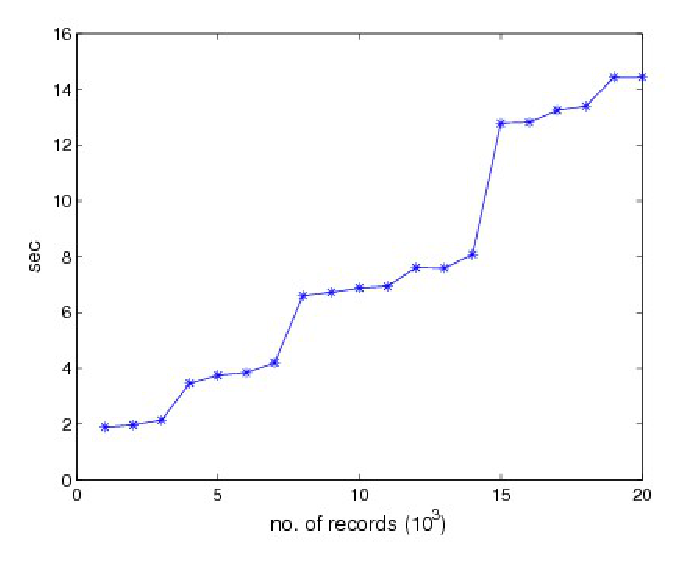
\includegraphics[width=0.98\textwidth]{phd_figures/dataSize.eps}
\caption{论文框架与技术路线,作者自绘。}\label{fig:Chapter1-lilun-kuangjia}
\vspace{\baselineskip} %表示图与正文空一行
\end{figure}

\subsection{创新点}

本研XXXX。








% !Mode:: "TeX:UTF-8"

\chapter{特大XXX}

XXX。


\section{实测场地选择XXX}\label{sec:test_describe_and_measurements}

本节XXXX。

\FloatBarrier
\section{计算机XXX}
\label{sec:simulation_discribe}

由XXX。

\FloatBarrier
\section{混响XXX}

XXX

\FloatBarrier
\section{本章小结}

本章的研究目的为XXX以后将对其做更深入研究。

% !Mode:: "TeX:UTF-8"

\chapter{特大空间声场的声XXXX}

本章旨在XXX。

\section{声能空XXX}

本节研究XXX。

\subsection{实测XXX}

天津党校报告XXX

 其平面图如图~\ref{fig:chapt_2_plan_HIT}所示,场地概况和测试环境描述同第\ref{sec:test_describe_and_measurements} 节。

a)测试设备:测试中所用声源为无指向球形声源声望OS002,位于比赛场地中央略偏$\rm 1m$位置,离地高度为$\rm 1.5m$。

\subsection{计算XX}

XXXX

其他未说明的模拟设置与章节\ref{sec:simulation_discribe}相同。


\subsection{模拟结果分析}

XXX。

XXXX
\begin{equation}
\label{classical_equation}
L^c=10log_{10}(\frac{W}{4{\pi}r^2}+\frac{4W}{R})+120
\end{equation}

单位为$\rm dB$。其中,$\rm L^c$为室内声压级经典计算公式的计算结果;$\rm W$为声源声功率(W);$\rm R$为房间常数;$\rm r$为距声源距离($\rm m$)。
XXX

\begin{table}[!htb]
\centering
\caption{不同容积下的降噪曲线线性回归}
\label{tab:chapt_3_regression_noise_reduction}
\vspace{0.5em}\centering\wuhao
\begin{tabular}{cccccccc}
\toprule[1.5pt]
\multirow{2}{*}{空间类型}                                               & \multirow{2}{*}{回归结果} & \multicolumn{6}{c}{空间宽度(m)}                         \\
                                                                    &                                   & 20     & 40     & 60     & 80     & 100    & 150    \\ \midrule[1pt]
\multirow{2}{*}{类型~\uppercase\expandafter{\romannumeral1}} & 斜率                             & -10.02 & -9.93  & -9.53  & -9.11  & -8.73  & -7.95  \\
                                                                    & $R^2$                                & 0.954  & 0.971  & 0.98   & 0.986  & 0.989  & 0.995  \\
\multirow{2}{*}{类型~\uppercase\expandafter{\romannumeral2}} & 斜率                             & -14.6  & -14.06 & -13.46 & -12.93 & -12.46 & -11.49 \\
                                                                    & $R^2$                                & 0.974  & 0.982  & 0.986  & 0.99   & 0.992  & 0.995  \\
\bottomrule[1.5pt]
\end{tabular}
\vspace{\baselineskip}
\end{table}

\subsection{不均匀XXX}


\FloatBarrier
\section{本章小结}
本章的研究目XXX。

% !Mode:: "TeX:UTF-8"

\chapter{特XXXX}

本章研究旨在XXX具有十分重要的理论意义和现实意义。


\section{人群噪XXXX}

本节研究旨在XXXX准确性。

\subsection{实地测试}
本文XXX。
xxx
XXXX
\FloatBarrier
\section{本章小结}
本章XXX。

% !Mode:: "TeX:UTF-8"

\chapter{特大XXX}

本文通过XXX。

\section{XX设计策略}

XXX。

\subsection{空间体XX}

本文XXX的。


\subsection{界面XXX}

XXX。

\section{本章小结}

本章节XXX。


% !Mode:: "TeX:UTF-8"
\setcounter{secnumdepth}{-2}
%\addcontentsline{toc}{chapter}{结\quad 论} %添加到目录中
\chapter{结\quad 论 \quad 和\quad 展\quad 望}
\markboth{结\quad 论 \quad 和\quad 展\quad 望}{结\quad 论 \quad 和\quad 展\quad 望}

\section*{结论}
本文通过对特大空XXXXX。

\section*{不足和展望}

本文的研究XXX。分别论述如下:

(1)XXX。

(2)XXX。

(3)XXX。

这些都有待进一步的研究和探索。

%%%%%%%%%% 正文部分内容  %%%%%%%%%%

%%%%%%%%%%  参考文献  %%%%%%%%%%
\setcounter{secnumdepth}{-2}
\chapter{参考文献}
\defaultfont
\bibliographystyle{GBT7714-2005NLang-TJU}
%\phantomsection
\markboth{参考文献}{参考文献}
%\addcontentsline{toc}{chapter}{参考文献}            % 参考文献加入到中文目录
%\nocite{*}                                          % 若将此命令屏蔽掉,则未引用的文献不会出现在文后的参考文献中。
\bibliography{references/reference_phd}
% !Mode:: "TeX:UTF-8"

\setcounter{secnumdepth}{-2}
%\addcontentsline{toc}{chapter}{发表论文和参加科研情况说明}
\chapter{发表论文和参加科研情况说明}
\markboth{发表论文和参加科研情况说明}{发表论文和参加科研情况说明}
\setlength{\parindent}{0em}

\textbf{(一)发表的学术论文}
\begin{publist}
\item  Wang, Chao, Hui Ma, Yue Wu, and Jian Kang. "Characteristics and prediction of sound level in extra-large spaces." Applied Acoustics 134 (2018): 1-7.(SCI二区)

\end{publist}

%\vspace*{1em}
\textbf{(二)申请及已获得的专利}
\begin{publist}
\item 马蕙;王超. 一种适用于钢结构建筑的非承重装配式隔声隔墙:中国,CN107419827A[P]. 2017-12-01.

\end{publist}
%\vspace*{1em}
\textbf{(三)参与的科研项目}
\begin{publist}
\item	2014年至今. 特大空间中声学引导人群疏散模型研究, ~国家自然科学基金项目.课题编号:51378139.
%\item	因校盲审要求隐去此部分
\end{publist}
\vfill
\hangafter=1\hangindent=2em\noindent

\setlength{\parindent}{2em}
                     % 发表论文和参加科研情况说明
% !Mode:: "TeX:UTF-8"

\setcounter{secnumdepth}{-2}
%\addcontentsline{toc}{chapter}{附\quad 录\quad A} %添加到目录中
\chapter{附\quad 录\quad A}
\markboth{附\quad 录\quad A}{附\quad 录\quad A}
\begin{center}
\large
计算机代码
\vspace{0.5cm}
\end{center}

镜像声源法python实现的核心代码如下:
\begin{verbatim}
import math
import numpy

class ImageMethod(object):
	def __init__(self):
		pass

\end{verbatim}

% !Mode:: "TeX:UTF-8"

\setcounter{secnumdepth}{-2}
%\addcontentsline{toc}{chapter}{致\quad 谢} %添加到目录中
\chapter{致\quad 谢}

\markboth{致\quad 谢}{致\quad 谢}

四年的XXX

\rightline{2018年X月XX日于天津}






                 % 致谢
\clearpage
\end{CJK*}                                          % 结束中文字体使用
\end{document}                                      % 结束全文
